\documentclass[10pt]{article}

\usepackage[T1]{fontenc}
\usepackage[utf8]{inputenc}
\usepackage{lmodern}
\usepackage[margin=0.7in]{geometry}
\usepackage{microtype}
\usepackage{enumitem}
\usepackage{booktabs}
\usepackage{tabularx}
\usepackage{array}
\usepackage{graphicx}
\usepackage{float}
\usepackage{xcolor}
\usepackage{tikz}
\usetikzlibrary{arrows.meta, positioning}
\usepackage{titlesec}
\usepackage[font=footnotesize, labelfont=bf, skip=3pt]{caption}
\usepackage[colorlinks=true, linkcolor=black, urlcolor=blue!60!black, citecolor=black]{hyperref}

% Compact layout so the proposal fits on two pages
\setlist{itemsep=0pt, topsep=1pt, parsep=0pt, leftmargin=1.4em}
\setlength{\parskip}{3pt}
\setlength{\parindent}{0pt}
\setlength{\intextsep}{5pt}
\titleformat*{\section}{\normalsize\bfseries}
\titlespacing*{\section}{0pt}{5pt}{0pt}
\newcolumntype{Y}{>{\raggedright\arraybackslash}X}

\begin{document}

\begin{center}
  \vspace*{-2.2em}
  {\Large\bfseries Player Archetypes in Competitive Disc Golf}\\[3pt]
  {\large\bfseries Project Proposal: CSYS 6870 Data Science II}\\[3pt]
  Luc Cohen-Wanis \quad$\cdot$\quad October 6, 2026
\end{center}
\vspace{-0.4em}

I'd like to identify play style archetypes among competitive disc golfers, specifically Disc Golf Vermont Tour (DGVT) players, from hole by hole scores (using tournament data from 2019-2026), estimate how hole design favors each style, and test whether styles improve score prediction beyond player rating.

% ---------------------------------------------------------------------------
\section{Research question}

\textbf{Do competitive disc golfers fall into distinct playing styles beyond overall skill, and do those styles explain and predict how players score on different kinds of holes?}

\textbf{Why it's interesting.}
Every competitive disc golfer has a PDGA rating, a single number meant to represent their skill and used to decide which divisions they can play in. But a rating doesn't say anything about how a player arrives at their score. One player might par every hole and finish even. Another might also finish even, but with six birdies and six bogeys, gaining strokes on long par 4s and giving them back on short, technical holes that reward good short game. I want to use player x hole x round data from the DGVT to test whether differences like these form consistent playing styles. If they do, disc golfers could see which archetype they fit and what it suggests they should work on.

\textbf{Related work.}
In golf, \emph{strokes gained} [1] scores every shot against a field baseline,
and I use the same idea at the hole level. In basketball, clustering NBA
players on their stats found 13 playing types instead of the 5 traditional
positions [2], which is similar to the archetype question. For disc golf,
\href{https://statmando.com/stats/}{StatMando} publishes stats for touring pros, but I haven't found any work on playing styles for amateur or regional players.

% ---------------------------------------------------------------------------
\section{Data collection, cleaning, and exploration}

The individual unit of analysis is one player on one hole in one round. PDGA Live has the hole by hole scores plus the par and length of every hole on each layout, and a player's PDGA rating at the time of the event gives me their overall skill.
I've already scraped PDGA results for 11 of 12 events of the 2026 tour (the final event is this weekend), and a handful of other events from previous years. To check that the hole level data is usable I explored one 2026 event in full: DGVTour \#9, the Kingdom Open (August 22-23, Lyndonville, VT). It has 104 players in 17 divisions over two rounds, which gives 3,708 player x hole scores, and the hole scores add up to the official round score in all 206 completed rounds.

From the raw scores I'll build the following features:
\begin{itemize}
  \item \emph{strokes gained}: the field's average score on a hole minus the player's score
  \item \emph{style-adjusted}: version that subtracts the player's own average so it shows where they gain and lose strokes instead of how many
  \item \emph{hole types}: short, medium or long within each par
\end{itemize}

Things that I've observed from exploring the data so far:
\begin{itemize}
  \item Older events may not have hole by hole scores: my first step will be determining what events are usable.
  \item Divisions play different tees so the field average has to be computed per layout, not per division.
  \item Unfinished rounds are stored as a round score of 999, but are still marked as completed.
  \item Hole length isn't everything: two par 4s that have similar distances can score very differently across the field.
\end{itemize}

% ---------------------------------------------------------------------------
\section{Analysis plan}

\textbf{Descriptive: what styles exist?}
For each player my goal is to build a style profile: strokes gained by hole type, their mix of birdies, pars, bogeys and worse, and how much they vary from round to round. Then, I'll cluster the profiles and check that the clusters hold up from one season to the next. Figure~\ref{fig:prelim} is a first look from the Kingdom Open: players with similar ratings and the same final score at an event can have different mixes of birdies and big numbers.

\suppressfloats[t]
\begin{figure}[t]
\centering
\begin{minipage}[t]{0.42\textwidth}
  \centering
  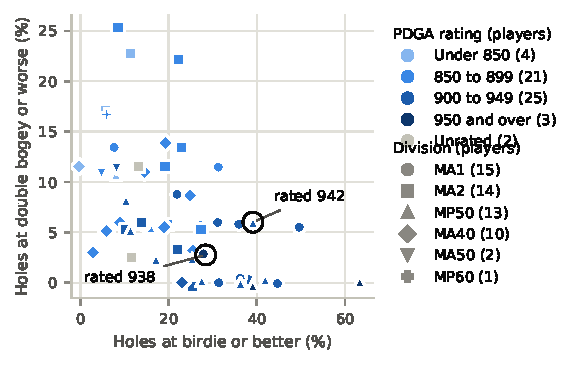
\includegraphics[width=\linewidth]{figures/preliminary_figure.pdf}
  \caption{Birdie rate against double-bogey-or-worse rate for the 55 players on the Kingdom Open Blue tees (36 holes each). Color shows rating band and shape shows division. The two circled MP50 players, rated 938 and 942, both finished 4 under par: one with 10 birdies, the other with 14.}
  \label{fig:prelim}
\end{minipage}\hfill
\begin{minipage}[t]{0.55\textwidth}
  \centering
  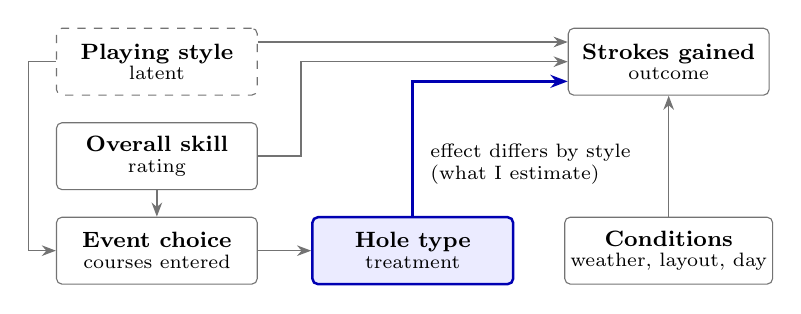
\begin{tikzpicture}[
      box/.style={draw=black!55, rounded corners=2pt, minimum width=2.55cm,
                  minimum height=0.85cm, align=center, font=\footnotesize,
                  inner sep=2pt},
      latent/.style={box, dashed},
      treat/.style={box, draw=blue!70!black, fill=blue!8, line width=0.9pt},
      arr/.style={-{Stealth[length=1.8mm]}, draw=black!55, line width=0.5pt},
      eff/.style={-{Stealth[length=2.2mm]}, draw=blue!70!black, line width=1pt}
    ]
    \node[latent] (style)   at (0, 2.7)   {\textbf{Playing style}\\[-2pt]\scriptsize latent};
    \node[box]    (skill)   at (0, 1.5)   {\textbf{Overall skill}\\[-2pt]\scriptsize rating};
    \node[box]    (event)   at (0, 0.3)   {\textbf{Event choice}\\[-2pt]\scriptsize courses entered};
    \node[treat]  (hole)    at (3.25, 0.3){\textbf{Hole type}\\[-2pt]\scriptsize treatment};
    \node[box]    (outcome) at (6.5, 2.7) {\textbf{Strokes gained}\\[-2pt]\scriptsize outcome};
    \node[box]    (cond)    at (6.5, 0.3) {\textbf{Conditions}\\[-2pt]\scriptsize weather, layout, day};

    \draw[arr] ([yshift=2.5mm]style.east) -- ([yshift=2.5mm]outcome.west);
    \draw[arr] (skill.east) -- ++(0.55, 0) |- (outcome.west);
    \draw[arr] (style.west) -- ++(-0.35, 0) |- (event.west);
    \draw[arr] (skill.south) -- (event.north);
    \draw[arr] (event.east) -- (hole.west);
    \draw[eff] (hole.north) |- ([yshift=-2.5mm]outcome.west);
    \draw[arr] (cond.north) -- (outcome.south);

    \node[align=left, font=\scriptsize, anchor=west] at (3.35, 1.4)
        {effect differs by style\\(what I estimate)};
  \end{tikzpicture}
  \caption{Causal diagram. Everyone in a division plays the same holes each
  round, so style and skill only affect which hole types a player faces through
  the events they choose to enter.}
  \label{fig:dag}
\end{minipage}
\end{figure}

\textbf{Explanatory: does hole design favor some styles?}
The treatment is the hole type (for example long vs short), the outcome is a
player's strokes gained on that hole, and what I want to estimate is how the
effect of hole type changes with playing style. I'd like to use a mixed-effects model with player effects, hole-by-round effects, and style x hole type interactions. The key assumption (Figure~\ref{fig:dag}) is that within a round everyone in a division plays the same holes, so a player only ``chooses'' hole types by choosing which events to enter, and player effects account for that. To avoid testing a style on the scores that defined it, I'll assign styles on 2019-2023 events and estimate the effects on 2024-2026 events.

\textbf{Predictive: do styles carry information?}
I'll predict the score category (birdie or better, par, bogey, double bogey or worse) for each player on each hole of held-out events, and compare a model that only knows rating and hole difficulty against one that also knows the player's style. At the Kingdom Open, for instance, these categories were 21\%, 51\%, 21\% and 8\% of scores, so there's enough of each to model. My hope is that style improves predictions on events the model hasn't seen, which might be evidence the archetypes are real and not just noise from the clustering.

% ---------------------------------------------------------------------------
\section{Engineering plan}

The project will be a Python package in one GitHub repo with four stages: (1) scrape, saving the raw PDGA pages so pages don't get scraped twice, (2) parse and clean into tidy tables, with checks like hole scores adding up to round totals, (3) build features (strokes gained, hole types, style profiles), and (4) analyze the data in jupyter notebooks. The repo will have a README, a license and documentation.

% ---------------------------------------------------------------------------
\section{Needs assessment and contingency plan}

\textbf{What I need to learn/review.}
How to choose and validate clusters (mixture models, BIC, stability) and how to fit mixed-effects models where players are crossed with holes.

\textbf{What could go wrong.}
\begin{itemize}
  \item Too few events have hole by hole scores. I'd add other Vermont
        events or maybe fall back to round-level features.
  \item The clusters just recover skill. I'll subtract each player's average
        and report how closely the clusters track rating.
  \item There aren't distinct groups. I might report continuous style dimensions
        and not call them archetypes.
  \item Players pick courses that suit them. Player effects handle part of
        this, and my estimates only apply to players who showed up.
\end{itemize}

\textbf{Minimum viable project.}
The player x hole table, strokes gained, style profiles, a validated clustering
(or style dimensions), a first estimate of how hole type changes each style's
advantage, and the prediction comparison.
\textbf{Stretch goals.}
Adding whether a bad hole carries over to the next one, and applying the same pipeline to players on the Disc Golf Pro Tour.

% ---------------------------------------------------------------------------
\section{Timeline}

\begin{table}[H]
\centering
\footnotesize
\setlength{\tabcolsep}{4pt}
\renewcommand{\arraystretch}{0.92}
\begin{tabularx}{\textwidth}{@{}p{1.25cm}Y>{\raggedright\arraybackslash}p{5.7cm}@{}}
\toprule
\textbf{Week of} & \textbf{Work} & \textbf{Deliverable} \\
\midrule
Oct 5  & Count which events have hole by hole scores; preliminary figure &
  Proposal (Oct 6) \\
Oct 12 & Scrape hole scores and layouts for all events; check against round totals &
  Clean player x hole table \\
Oct 19 & Strokes gained, hole types, style profiles, first clustering &
  Descriptive figures \\
Oct 26 & Write up the check-in: clean table, strokes gained by hole type, first clustering &
  \textbf{Halfway check-in (Oct 27)} \\
Nov 2  & Check cluster stability (bootstrap, season to season, against rating) &
  Final archetypes or style dimensions \\
Nov 9  & Style x hole type model on 2024-2026 events & Explanatory results \\
Nov 16 & Held-out score prediction with and without style & Predictive results \\
Nov 23 & Buffer (Thanksgiving); stretch goals; README, license, docs &
  Clean up repo \\
Nov 30 & Write the final report & Report draft \\
Dec 7  & Submit the report and present &
  \textbf{Report (Dec 8), presentation (Dec 9)} \\
\bottomrule
\end{tabularx}
\end{table}

% ---------------------------------------------------------------------------
{\footnotesize
\textbf{References.}
[1] M.~Broadie. Assessing golfer performance on the PGA TOUR.
\emph{Interfaces}, 42(2):146--165, 2012.
[2] M.~Alagappan. From 5 to 13: Redefining the positions in basketball.
\emph{MIT Sloan Sports Analytics Conference}, 2012.
}

\end{document}